\chapter{Data Samples and Monte Carlo Simulation}\label{samples}

\section{Trigger and data samples}

\par The data employed for this search were collected by the CMS experiment at $\sqrt{s} = 13$ TeV, and correspond to a total integrated luminosity of 2.3 {\fbinv}.
Signal event candidates are recorded online using a trigger designed to select $\HT^{\text{miss}}$ and $\MET$ with a lower threshold of 90 GeV in each case.
The $\HT^{\text{miss}}$ is computed as the magnitude of a vectorial sum of the transverse momenta of all jets with  $\pt$ greater than 20 GeV.
To reject events arising from atypical detector performance, supplementary selection requirements are set on the jets used in the $\HT^{\text{miss}}$ calculation.
The $\MET$ is defined as the magnitude of the negative vectorial sum of the transverse momentum of all the particles identified at the trigger level.
Identified muons are removed from the event before the $\MET$ and $\HT^{\text{miss}}$ are calculated.
And additional support trigger was used in combination with the main signal trigger. This trigger select events that contains $\MET$ with a lower threshold of 170 GeV. Selected events are required to have $\MET >$ 250 GeV to guarantee a trigger efficiency greater than 98$\%$ for all events used in the analysis. The trigger paths are reported in the Table \ref{tab:triggerPaths}. For additional information about the trigger paths and the efficiency calculation, we refer the reader to the Appendix \ref{appendix:ApendiceA}.

\begin{table}[!ht]
\footnotesize
\begin{center}
\caption{HLT Trigger path with their respective criteria.}
\label{tab:triggerPaths}
\begin{tabular}{cc} \hline
Trigger path & Criteria  \\ \hline
\verb|PFMETNoMu90_JetIdCleaned_PFMHTNoMu90_IDTight| (unprescaled)  &  $\MET>$ 90 GeV, $H_{\text{T}}^{\text{miss}}>$ 90 GeV\\
\verb|PFMET170_*| (unprescaled)  &  $\MET>$ 170 GeV \\ \hline
\end{tabular}
\end{center}
\end{table}

We use about 2.3 fb$^{-1}$ of data collected during the Run2015C and Run2015D era (Table \ref{tab:datasamples}) and reconstructed with the CMSSW 7 6 X release. We employ only lumisections that have been declared good for analysis by the central certification team.

\begin{table}[!ht]
\begin{center}
\caption{Data samples.}
\label{tab:datasamples}
\begin{tabular}{cc} \hline
Sample & Number of events  \\ \hline
\verb|MET/Run2015D| & 17996789   \\
\verb|MET/Run2015C| & 106269  \\ \hline
\end{tabular}
\end{center}
\end{table}


\section{Simulated Samples}

The analysis makes use of various simulated event samples for modeling the SM background and signal processes. A benchmark model, the bulk graviton (spin-2), is used to illustrate typical signal behavior. Simulated signal samples of bulk graviton resonances decaying to dibosons (ZZ) and subsequently to quarks and neutrinos are generated at leading order (LO) with the $\MADGRAPH 5$ \cite{Alwall:2014hca}  program interfaced with $\PYTHIA$8 \cite{Sjostrand:2006za,Sjostrand:2007gs} for the parton showering and hadronization, considering a coupling constant $\tilde{k}$ = 0.5. For this model we considered defined values of the resonances mass in the range 0.8 $ \leq m_{X} \leq $ 2 TeV in steps of 100 GeV. We restrict the analysis to scenarios where the natural width of the resonance is sufficiently small to be neglected when compared to the detector resolution. This makes our modelling of the detector effects on the signal shape independent of the actual model used for generating the events. The signal samples used in the analysis are shown in Table \ref{tab:signalsamples}.

\par Simulated samples are produced for the Z+jets, W+jets, $t\bar{t}$, dibosons and QCD multijet processes in order to describe the contribution expected from SM backgrounds. The main components of the total background are represented by Z + jets ($Z \rightarrow \nu \bar{\nu}$) and W+ jets ($W \rightarrow \ell \nu$) production. These as well as the QCD multijets sample, are simulated with $\MADGRAPH 5$ in LO mode and matched to $\PYTHIA$8 using the CUETP8M1 tune for hadronization and fragmentation. Double counting by the matrix element calculation and parton showering is resolved by using the MLM matching prescription \cite{Mangano:2002ea}. The SM background contribution from $t\bar{t}$ events is modeled at next-to-leading order (NLO) with the $a\MCATNLO$ program \cite{Frixione:2002ik}, interfaced with $\PYTHIA$8. Inclusive non-resonant dibosons simulated samples (WW/WZ/ZZ) are generated at LO with $\PYTHIA$8. All the background samples used in this analysis are listed in Table \ref{tab:backgroundsamples}.

\par The V+jets simulated samples are rescaled using next-to-next-to-leading order (NNLO) QCD correction in the cross sections (Table \ref{tab:scalefactors}) and NLO QCD electroweak (EW) correction in the V boson $\pt$ domain (Fig. \ref{fig:EW}) \cite{Kallweit:2015dum}. 

\par Minimum bias events are included during the production of the simulated samples to account for contributions from additional proton-proton collisions (pileup) with the number of reconstructed primary vertices matching those in data. The simulation is corrected from perceptible differences between data and simulation in the trigger and identification/isolation efficiency of leptons (electrons, muons, taus), photons and jets originating from hadronization of bottom quarks (b-jets).

\par In all the simulated samples, the events are generated using the NNPDF 3.0~\cite{Ball:2011mu} set of parton distribution functions. The simulation of the detector response is modeled with the \GEANTfour package~\cite{Agostinelli:2002hh}.

\begin{table}[!ht]
\footnotesize
\begin{center}
\caption{Monte Carlo simulated signal samples for Bulk graviton model.}
\label{tab:signalsamples}
\begin{tabular}{lcc} \hline
Sample & Cross Section (pb) & $\text{N}_{\text{events}}$ \\ \hline
\verb|BulkGravToZZToZhadZinv_narrow_M-800_13TeV-madgraph| & 1.0 & 100000 \\
\verb|BulkGravToZZToZhadZinv_narrow_M-1000_13TeV-madgraph| & 1.0 & 99200 \\
\verb|BulkGravToZZToZhadZinv_narrow_M-1200_13TeV-madgraph| & 1.0 & 95800 \\
\verb|BulkGravToZZToZhadZinv_narrow_M-1400_13TeV-madgraph| & 1.0 & 100000 \\
\verb|BulkGravToZZToZhadZinv_narrow_M-1600_13TeV-madgraph| & 1.0 & 100000 \\
\verb|BulkGravToZZToZhadZinv_narrow_M-1800_13TeV-madgraph| & 1.0 & 98000 \\
\verb|BulkGravToZZToZhadZinv_narrow_M-2000_13TeV-madgraph| & 1.0 & 99200 \\
\verb|BulkGravToZZToZhadZinv_narrow_M-2500_13TeV-madgraph| & 1.0 & 99200 \\
\verb|BulkGravToZZToZhadZinv_narrow_M-3000_13TeV-madgraph| & 1.0 & 99600 \\
\verb|BulkGravToZZToZhadZinv_narrow_M-3500_13TeV-madgraph| & 1.0 & 100000 \\
\verb|BulkGravToZZToZhadZinv_narrow_M-4000_13TeV-madgraph| & 1.0 & 99200 \\
\verb|BulkGravToZZToZhadZinv_narrow_M-4500_13TeV-madgraph| & 1.0 & 99000 \\ \hline
\end{tabular}
\end{center}
\end{table}


\begin{table}[!ht]
\small
\begin{center}
\caption{Monte Carlo background samples.}
\label{tab:backgroundsamples}
\begin{tabular}{lcc} \hline
Sample & Cross Section (pb) & $\text{N}_{\text{events}}$ \\ \hline
$Z(\rightarrow \nu \bar{\nu})$+jets, $100 < \HT < 200$ GeV & 280.35 & 5240199 \\
$Z(\rightarrow \nu \bar{\nu})$+jets, $200 < \HT < 400$ GeV & 77.67 & 5135542 \\
$Z(\rightarrow \nu \bar{\nu})$+jets, $400 < \HT < 600$ GeV  & 10.73 & 954435  \\
$Z(\rightarrow \nu \bar{\nu})$+jets, $\HT > 600$ GeV & 4.116 & 1033818 \\ \hline
$W(\rightarrow \ell \nu)$+jets, $100 < \HT < 200$ GeV & 1345 & 10205377  \\
$W(\rightarrow \ell \nu)$+jets, $200 < \HT < 400$ GeV & 359.7  & 4949568  \\
$W(\rightarrow \ell \nu)$+jets, $400 < \HT < 600$ GeV & 48.91 & 1943664  \\
$W(\rightarrow \ell \nu)$+jets, $\HT > 600$ GeV & 18.77 & 1041358  \\ \hline
QCD multjets,$100 < \HT < 200$ GeV & 27990000  & 82095800 \\
QCD multjets,$200 < \HT < 300$ GeV & 1712000 & 18784379 \\
QCD multjets,$300 < \HT < 500$ GeV & 347700 & 16909004  \\
QCD multjets,$500 < \HT < 700$ GeV & 32100  & 19665695  \\
QCD multjets,$700 < \HT < 1000$ GeV& 6831  & 15547962 \\
QCD multjets,$1000 < \HT < 1500$ GeV & 1207 & 5049267 \\
QCD multjets,$1500 < \HT < 2000$ GeV & 119.9 & 3939077  \\
QCD multjets,$ \HT > 2000$ GeV & 25.24 & 1981228 \\ \hline
$t\bar{t}$ & 831.76 & 38475776 \\ 
$t\bar{t}$ (Extension) & 831.76 & 196937036 \\ \hline
$WW$ & 118.7 & 988418 \\
$WZ$ & 47.13  & 985600    \\
$ZZ$ & 16.523 & 996944 \\ \hline
\end{tabular}
\end{center}
\end{table}

\begin{table}[!ht]
\begin{center}
\caption{NNLO QCD flat scale factors.}
\label{tab:scalefactors}
\begin{tabular}{lc} \hline
Sample & Scale factor \\ \hline
Z + jets &  1.23   \\
W + jets  &  1.21\\ \hline
\end{tabular}
\end{center}
\end{table}

\begin{figure}[!ht]
\begin{center}
  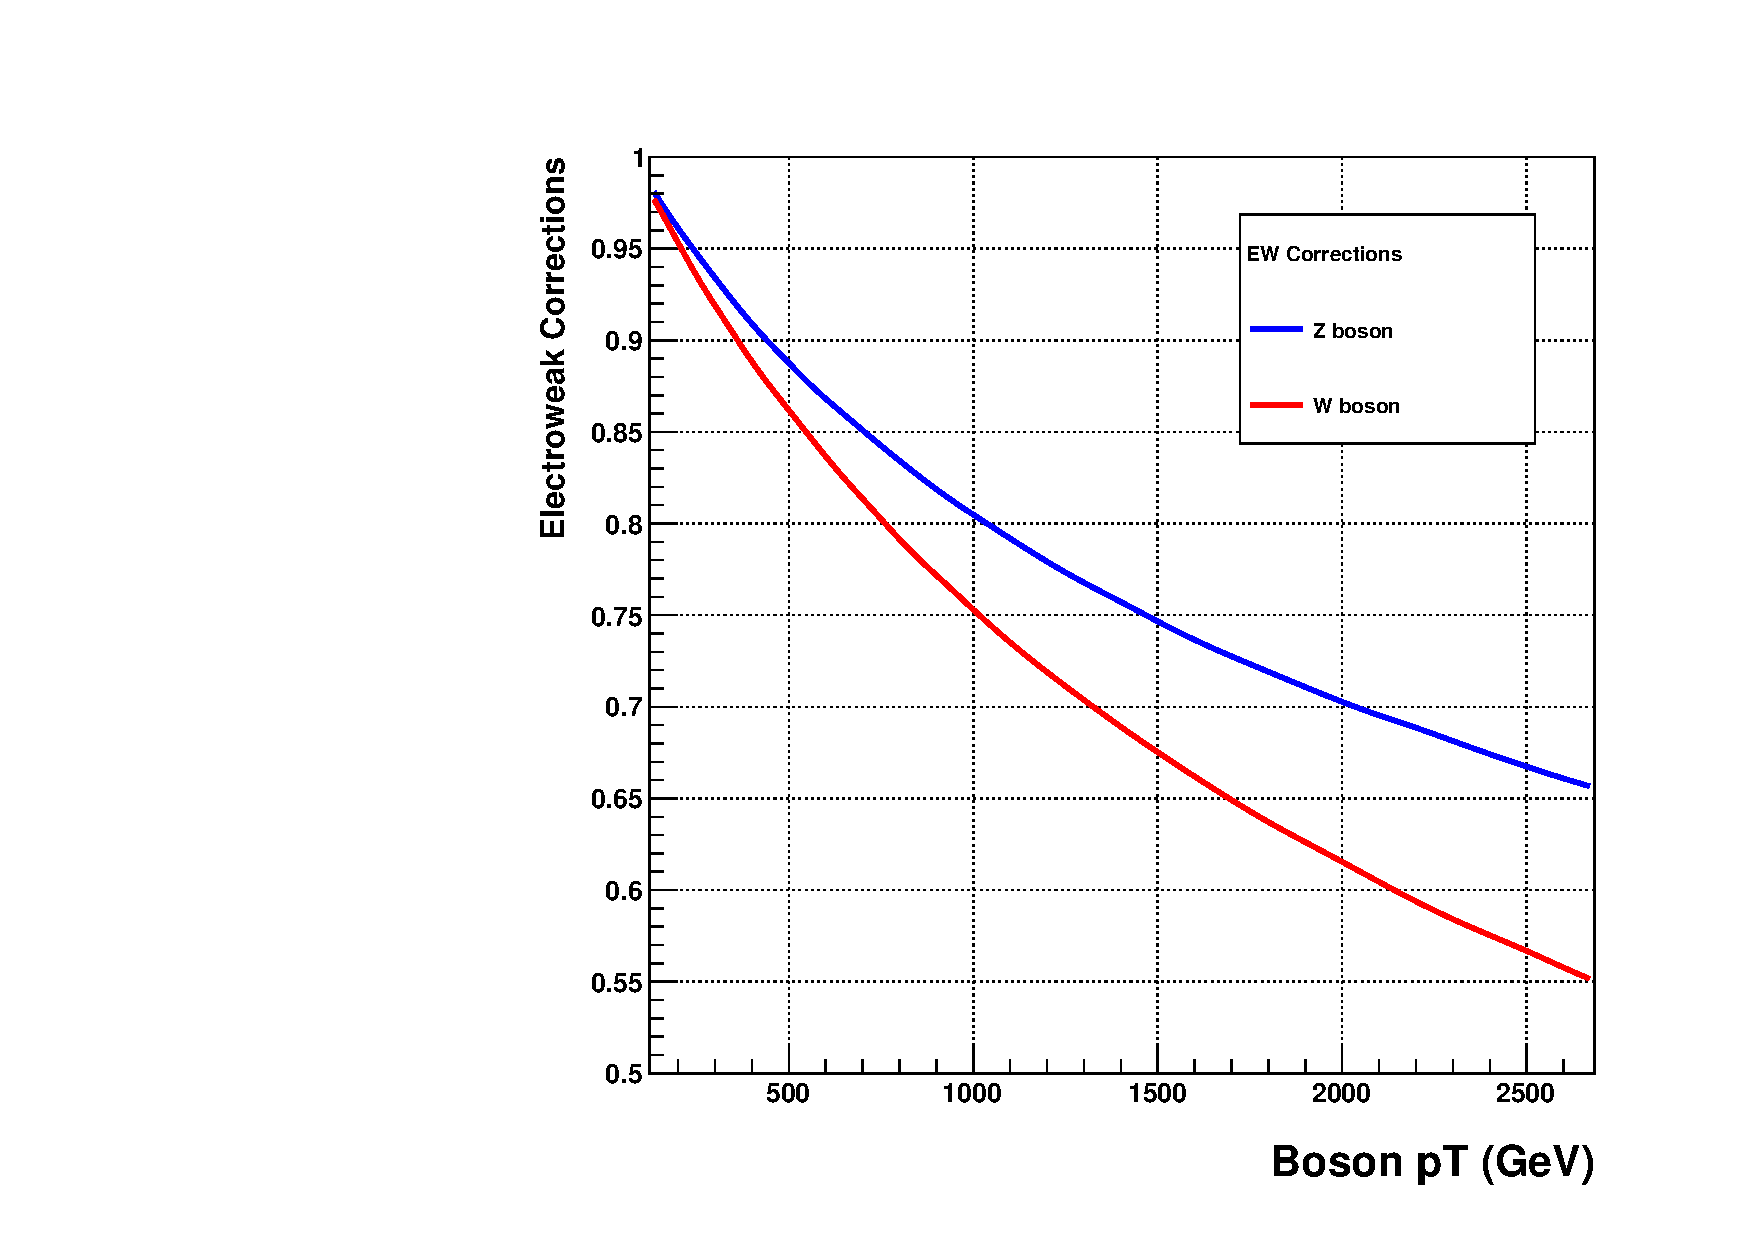
\includegraphics[width=240pt]{figures/Samples/EWcorrections.pdf}
\end{center}


\caption{Electroweak corrections for the W/Z boson in function of the boson $\pt$.}
\label{fig:EW}
\end{figure}

